\chapter{Seven Ways to Make a Full-Time Income While Traveling}

This chapter follows a School of Hard Knocks entrepreneurship lesson curated by LazyingArt LLC. The speaker's opening claim is deliberately simple: money can return, but time cannot. From that point the lecture asks a practical question: if travel matters now, what kinds of work let us earn without being tied to one fixed place? The answer is not one magic business model, but seven different mechanisms: selling skills, joining travel-based industries, building product margin, monetizing attention, packaging services, teaching language, and selling for large institutions.

\section{Travel, Time, and the Income Question}

The lecture begins with a contrast between two resources. Money is recoverable; time is not. That contrast gives the rest of the chapter its shape. We are not merely listing side hustles. We are asking which commercial arrangements make location less binding.

Let \(I\) denote income and let \(L\) denote location. A fixed-location job can be thought of as a strong dependence
\begin{equation}
I = I(L),
\end{equation}
where the earning mechanism is attached to one place. The lecture is interested in mechanisms where income is less dependent on physical location:
\begin{equation}
I \approx I(\text{skill},\text{offer},\text{market}),
\end{equation}
with location becoming a secondary variable rather than the center of the model.

That is the governing question: what has to be packaged, sold, or joined so that earning can continue while the person moves?

\section{Freelancing: A Skill Becomes a Remote Offer}

The first answer is freelancing online. The speaker names familiar platforms such as Fiverr and Upwork, but the real point is not the platform itself. The point is that a skill can become a remote offer when a customer already needs the service and the work can be delivered digitally.

The transcript moves through examples quickly: writing, graphic design, editing photography, editing YouTube videos, editing TikToks, social media management, running Google ads, running Facebook ads, creating content, and creating static posts. The shared structure is the same in each case:
\begin{equation}
\text{Portable service}
=
\text{skill}
+
\text{client need}
+
\text{remote delivery}.
\end{equation}

The low-friction character of freelancing matters. We do not need a warehouse, a lease, or a formal company before the first transaction. We need a skill that can be described clearly enough for a buyer to understand what is being sold.

\begin{figure}
\centering
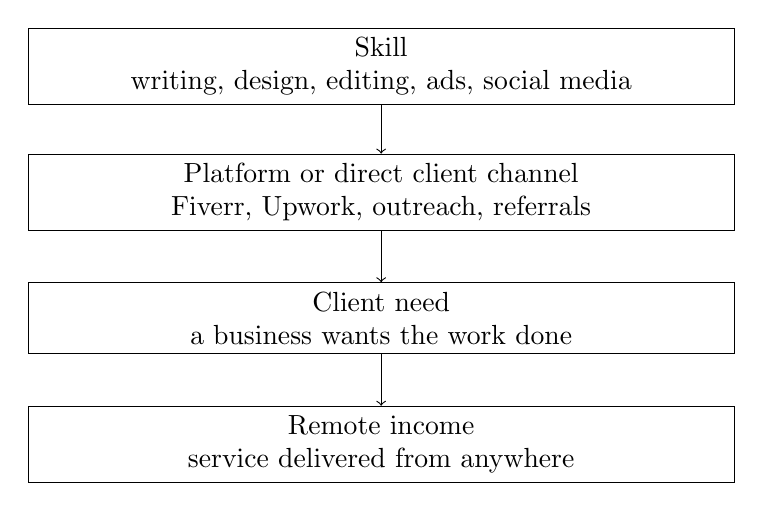
\begin{tikzpicture}
\node[draw, align=center, text width=0.72\linewidth] (skill) at (0,0) {Skill\\writing, design, editing, ads, social media};
\node[draw, align=center, text width=0.72\linewidth] (platform) at (0,-1.6) {Platform or direct client channel\\Fiverr, Upwork, outreach, referrals};
\node[draw, align=center, text width=0.72\linewidth] (client) at (0,-3.2) {Client need\\a business wants the work done};
\node[draw, align=center, text width=0.72\linewidth] (income) at (0,-4.8) {Remote income\\service delivered from anywhere};
\draw[->] (skill) -- (platform);
\draw[->] (platform) -- (client);
\draw[->] (client) -- (income);
\end{tikzpicture}
\end{figure}

The lecture's first move is therefore conservative: before we talk about brands, audiences, or institutions, we begin with the smallest commercial unit, a skill sold to someone who needs it.

\section{Hospitality: Getting Paid Inside the Travel System}

The second path changes the mechanism. Freelancing carries work through the internet. Hospitality carries the worker through the travel system itself. The speaker names cruise ships, yacht crews, flight attendants, resorts, and international hotels.

This is a different dependency structure. The worker is not necessarily location-independent in the same sense as a freelancer. Instead, the job itself contains movement:
\begin{equation}
\text{Travel}
\subset
\text{job conditions}.
\end{equation}

The examples are concrete. A yacht or cruise ship might travel from Miami toward the Virgin Islands. A flight attendant may see different countries in Europe. A resort or international hotel can place a worker in the Bahamas or another desired location. The point is not ownership. The point is access: if the industry needs labor in places people want to go, then work can become the ticket into those places.

This beat is important because it broadens the chapter. Portable income is not only laptop work. Sometimes the better model is to join an industry where relocation, lodging, flight benefits, or movement are already part of the operating system.

\section{E-Commerce: Margin, Storefront, and Distribution}

The third path introduces the clearest arithmetic in the lecture. The speaker says to find a product, whether through dropshipping or a manufacturer, and then sell it under an e-commerce brand. The example is t-shirts: perhaps the product costs roughly five, ten, or fifteen dollars, and sells for roughly twenty, twenty-five, or thirty dollars.

Let \(C\) be the unit cost and \(P\) the sale price. The transcript gives the cost and price ranges as
\begin{align}
C &\in \{\$5,\ \$10,\ \$15\},\\
P &\in \{\$20,\ \$25,\ \$30\}.
\end{align}

The simplest gross profit per unit is
\begin{equation}
\pi = P-C.
\end{equation}

If we use the speaker's phrase ``return on investment'' in a cautious unit-level sense, then a simple reconstruction is
\begin{equation}
\mathrm{ROI} = \frac{P-C}{C}.
\end{equation}
This is not a full accounting model. It leaves out ads, fulfillment, shipping, platform fees, refunds, taxes, and labor. But it captures the spoken mechanism: the entrepreneur looks for a spread between what the product costs and what the market will pay.

\subsection{Question \& Answer}

\paragraph{Question.}
What makes this more than simply buying low and selling high?

\paragraph{Answer.}
The lecture answers by moving immediately from price to distribution. The t-shirt example is only the arithmetic core. A brand also needs a product, a supplier or manufacturer, possibly a designer, an accessible storefront such as Shopify, and a way to reach buyers through Google, Facebook, TikTok, Instagram, branded content, or viral content. The margin is necessary, but it is not the whole business.

\subsection{A Worked Unit Example}

Take a cautious example close to the transcript. Suppose a shirt costs
\[
C=\$10
\]
and sells for
\[
P=\$25.
\]
Then the gross profit per unit is
\begin{align}
\pi &= P-C\\
&= \$25-\$10\\
&= \$15.
\end{align}
The simple unit-level return is
\begin{align}
\mathrm{ROI}
&= \frac{P-C}{C}\\
&= \frac{15}{10}\\
&= 1.5.
\end{align}
So before the omitted costs, the unit produces a gross return of \(150\%\) on the unit cost. The lecture's practical warning is implicit: that number only becomes a business if the product can be sourced reliably and sold repeatedly through a working marketing channel.

\begin{figure}
\centering
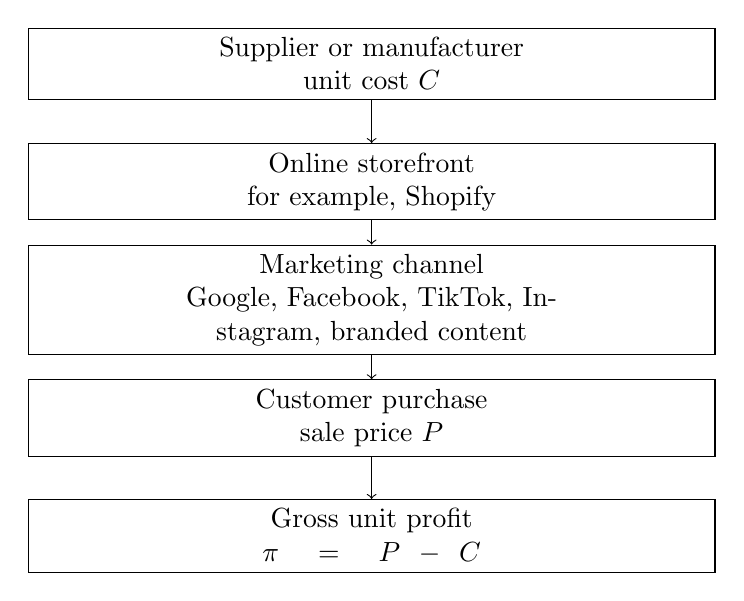
\begin{tikzpicture}
\node[draw, align=center, text width=0.70\linewidth] (source) at (0,0) {Supplier or manufacturer\\unit cost \(C\)};
\node[draw, align=center, text width=0.70\linewidth] (store) at (0,-1.5) {Online storefront\\for example, Shopify};
\node[draw, align=center, text width=0.70\linewidth] (market) at (0,-3.0) {Marketing channel\\Google, Facebook, TikTok, Instagram, branded content};
\node[draw, align=center, text width=0.70\linewidth] (sale) at (0,-4.5) {Customer purchase\\sale price \(P\)};
\node[draw, align=center, text width=0.70\linewidth] (profit) at (0,-6.0) {Gross unit profit\\\(\pi=P-C\)};
\draw[->] (source) -- (store);
\draw[->] (store) -- (market);
\draw[->] (market) -- (sale);
\draw[->] (sale) -- (profit);
\end{tikzpicture}
\end{figure}

The speaker then widens the example: it does not have to be t-shirts. It can be any product. The chapter should preserve that widening because it marks the transition from one example to the broader e-commerce mechanism.

\section{Content Creation: Audience Before Departure}

The fourth path is introduced as the most fun way to get paid to travel: becoming a content creator. But the lecture immediately adds a constraint. The speaker warns that if someone leaves with little money and no following, hoping to build everything from scratch in a new country or island, there is a real chance of running out of money quickly.

That warning is the center of the section. The income mechanism is not simply travel plus camera. It is audience-mediated monetization:
\begin{equation}
\text{Creator income}
=
f(\text{audience},\text{trust},\text{offers},\text{brand demand}).
\end{equation}

\subsection{Question \& Answer}

\paragraph{Question.}
Can we build the audience after we arrive?

\paragraph{Answer.}
The transcript's answer is cautious. Build the base first. A following gives brands a reason to pay for promotion, and it gives the creator a better chance of earning from the content being posted. Travel can supply material, but the audience is the asset that makes the material commercially useful.

The lecture lists several creator income channels: affiliate relationships, selling one's own products, merchandise, launching an e-commerce brand, travel blogging, working with brands, and becoming a brand ambassador. A simple affiliate model is
\begin{equation}
I_{\mathrm{affiliate}} = r S_{\mathrm{referred}},
\end{equation}
where \(r\) is the commission rate and \(S_{\mathrm{referred}}\) is the value of referred sales. This formula is a reconstruction of the phrase ``take a percentage of their sales,'' not a displayed equation from the lecture.

The speaker also gives a concrete claim: some long-term ambassador programs may pay about
\begin{equation}
A \approx \$10{,}000\text{--}\$20{,}000
\end{equation}
for a series of paid advertisements. We should keep that as a claim from the interview context, not as a guaranteed market rate.

\section{Agencies: Packaging Expertise for Clients}

The fifth path is starting an agency. This is close to freelancing, but it has a different commercial shape. A freelancer sells a task or skill. An agency packages a capability so that brands and companies can buy an outcome or ongoing service.

The lecture names photography, digital marketing, social media growth, programming, and written software for companies. These are all ways of converting skill into an offer:
\begin{equation}
\text{Agency offer}
=
\text{skill}
+
\text{packaging}
+
\text{client value}.
\end{equation}

The distinction between physical and remote work matters. If the agency must create on-location content, then travel may need to match the client's location. If the client only needs content strategy, programming, software, or social growth advice, then the work can remain remote. The practical question is not whether the skill is impressive. It is whether the service can be delivered at a distance without destroying the value promised to the client.

\section{Language Tuition and Sales: Institutional Demand}

The sixth path is language tuition. The speaker frames it as teaching English in countries where English instruction is in demand. The claim is not merely that teaching pays. It is that demand can be strong enough for some positions to cover relocation, housing, and income.

The mechanism here is institutional demand:
\begin{equation}
\text{Income}
=
\text{language ability}
+
\text{local demand}
+
\text{institutional placement}.
\end{equation}
The lecture names children, adults, schools, and teachers as possible learners or settings. The portable element is fluency, but the paying customer is often an institution or an organized education market.

The seventh and final path is sales representation. The speaker names information technology, defense, insurance, and pharmaceutical industries, all of which need strong salespeople to sell products or services to other companies. Here the commercial asset is not a product owned by the traveler. It is the ability to persuade, maintain relationships, and close business for an organization with something valuable to sell.

The transcript includes the claim that some large industries may pay
\begin{equation}
S > \$100{,}000
\end{equation}
annually to people who put in the work on the road. This should be written as a possibility in some industries, not as a general promise. The mechanism is high-ticket institutional selling, and the required asset is strong sales skill plus interpersonal relationship skill.

\section{The Seven Mechanisms Together}

The lecture is a list, but the list has an internal structure. We can classify the seven ways by the economic object being sold or used.

\begin{figure}
\centering
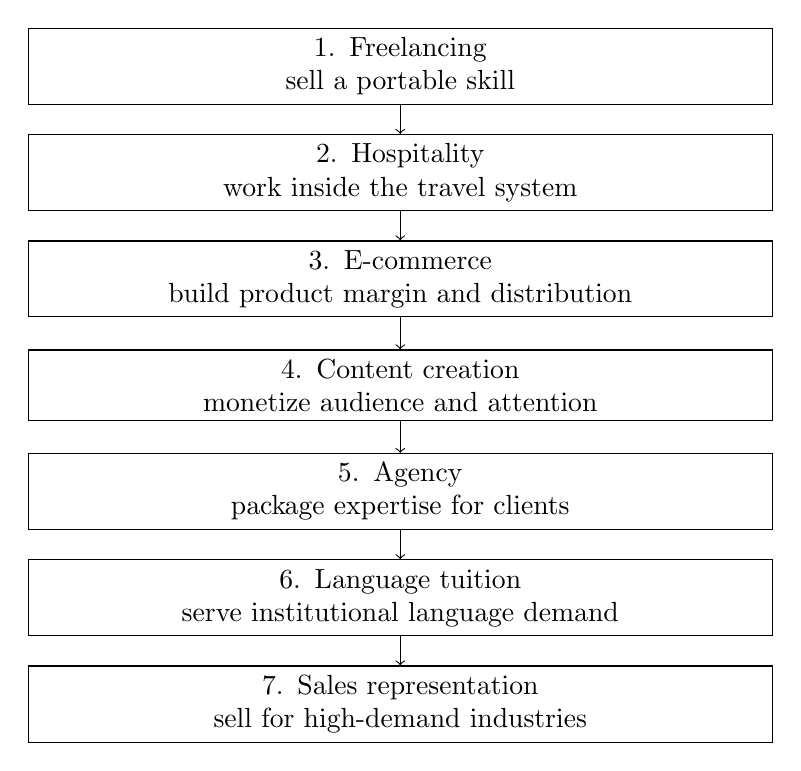
\begin{tikzpicture}
\node[draw, align=center, text width=0.76\linewidth] (a) at (0,0) {1. Freelancing\\sell a portable skill};
\node[draw, align=center, text width=0.76\linewidth] (b) at (0,-1.35) {2. Hospitality\\work inside the travel system};
\node[draw, align=center, text width=0.76\linewidth] (c) at (0,-2.70) {3. E-commerce\\build product margin and distribution};
\node[draw, align=center, text width=0.76\linewidth] (d) at (0,-4.05) {4. Content creation\\monetize audience and attention};
\node[draw, align=center, text width=0.76\linewidth] (e) at (0,-5.40) {5. Agency\\package expertise for clients};
\node[draw, align=center, text width=0.76\linewidth] (f) at (0,-6.75) {6. Language tuition\\serve institutional language demand};
\node[draw, align=center, text width=0.76\linewidth] (g) at (0,-8.10) {7. Sales representation\\sell for high-demand industries};
\draw[->] (a) -- (b);
\draw[->] (b) -- (c);
\draw[->] (c) -- (d);
\draw[->] (d) -- (e);
\draw[->] (e) -- (f);
\draw[->] (f) -- (g);
\end{tikzpicture}
\end{figure}

The order matters. The speaker begins with individual skills, moves to travel-embedded employment, then to product and audience systems, and finally to institutional demand. That is a useful progression for an entrepreneurship book because it separates seven names from seven mechanisms.

\begin{table}
\centering
\begin{tabular}{l l}
Path & Main economic asset \\
Freelancing & Remote skill sold to clients \\
Hospitality & Job access inside travel industries \\
E-commerce & Product margin plus distribution \\
Content creation & Audience and brand attention \\
Agency & Packaged expertise for companies \\
Language tuition & English ability and relocation demand \\
Sales representation & Sales skill in large industries \\
\end{tabular}
\end{table}

\section{Summary}

The lecture's promise is not that every path is easy or equally reliable. Its more useful claim is structural: location freedom can be built in several different ways. We can sell a skill remotely, join work that already moves, create product margin, build an audience, package expertise, teach where language demand is strong, or sell for institutions that pay for revenue.

The chapter's mathematics stays modest because the source material is practical rather than formal. Still, the arithmetic matters. In e-commerce, the unit spread \(P-C\) is the beginning of the story, not the end. In creator work, affiliate income depends on a rate and referred sales, but those depend on an audience built before the trip. In sales, a six-figure compensation claim depends on industry demand and the ability to perform on the road.

The final lesson is therefore commercial rather than motivational: travel becomes more feasible when income is attached to a portable asset. The asset may be a skill, a product, an audience, a client package, a language ability, or a sales capacity. The work is to know which asset we actually have, and which market will pay for it while we move.